\documentclass[10pt,letterpaper]{article} 
\usepackage{tikz}
\usepackage{toolsper}
%\usepackage{graphicx}‎‎
%\usefonttheme{serif}‎
%\usepackage{ptext}‎
%\usepackage{xepersian}
%\settextfont{B Nazanin}
\usepackage{lipsum}
\setlength{\parindent}{0pt}
\setlength{\parskip}{1em}
\newcommand{\pf}{$\blacksquare$}
\newcommand{\EX}{\Bbb E}
\newcommand{\nl}{\newline\newline}
\newcounter{QuestionNumber}
\setcounter{QuestionNumber}{1}

\newcommand{\wid}{40mm}
%\newcommand

\newcommand{\Q}{
\textbf{
سوال \theQuestionNumber)
}
\stepcounter{QuestionNumber}
}
\begin{document}
\large
\begin{center}
به نام زیبایی

پاسخ تمرینات سری دهم سیگنال ها و سیستم ها
\hl
\end{center}
\Q

الف)
\qn{
X(e^{j\omega})&=\sum_{n=-\infty}^\infty x[n] e^{-j\omega n}
\\&=\sum_{n=-\infty}^\infty (u[n]-u[n-5]) e^{-j\omega n}
\\&=\sum_{n=0}^4 e^{-j\omega n}
\\&=\begin{cases}
{1-e^{-5j\omega}\over 1-e^{-j\omega}}&,\quad \omega\ne 2k\pi
\\
5&,\quad \omega= 2k\pi
\end{cases}
}{}
ب)
\qn{
X(e^{j\omega})&=\sum_{n=-\infty}^\infty (1/3)^n u[n] e^{-j\omega n}
\\&=\sum_{n=0}^\infty (1/3e^{-j\omega})^n
\\&={1\over 1-1/3e^{-j\omega}}
}{}
زیرا 
$
|1/3e^{-j\omega}|<1
$
.

پ)
\qn{
X(e^{j\omega})&=\sum_{n=-\infty}^\infty -(1/3)^n u[-n-1] e^{-j\omega n}
\\&=\sum_{n=-\infty}^{-1} -(1/3e^{-j\omega})^n
\\&\notin \Bbb R
}{}
که وجود ندارد زیرا 
$
|1/3e^{-j\omega}|<1
$
 (دقت کنید که اندیس $n$ در این جمع منفی است)

ت) طبق خاصیت
\qn{
&\sin \omega_0 n \overset{F. T.}{\iff } {\pi\over j}\sum_{l=-\infty}^{\infty} [\delta(\omega-2\pi l -\omega_0)-\delta(\omega-2\pi l +\omega_0)]
\\&
\cos \omega_0 n \overset{F. T.}{\iff } {\pi}\sum_{l=-\infty}^{\infty} [\delta(\omega-2\pi l -\omega_0)+\delta(\omega-2\pi l +\omega_0)]
}{}
بنابراین
\qn{
X(e^{j\omega})&=
{\pi\over j}\sum_{l=-\infty}^{\infty} [\delta(\omega-2\pi l -{\pi\over 2})-\delta(\omega-2\pi l +{\pi\over 2})]
\\&+
{\pi}\sum_{l=-\infty}^{\infty} [\delta(\omega-2\pi l -1)+\delta(\omega-2\pi l +1)]
}{}
ث) طبق جدول خواص:
$$
nx[n]\iff j{d\over d\omega}X(e^{j\omega})
$$
بنابراین با کمک قسمت ب:
$$
X(e^{j\omega})={1/3e^{-j\omega}\over (1-1/3e^{-j\omega})^2}
$$
\Q

الف)
\qn{
X(e^{j\omega})&=\sum_{k=-\infty}^{\infty}(-1)^k\delta(\omega-{\pi\over 2}k)
\\&=\sum_{k=-\infty}^{\infty}\delta(\omega-{\pi}-2\pi k)
\\&-\sum_{k=-\infty}^{\infty}[\delta(\omega-{\pi\over 2}-2\pi k)+\delta(\omega+{\pi\over 2}-2\pi k)]
\\&+\sum_{k=-\infty}^{\infty}\delta(\omega-2\pi k)
}{}
بنابراین
$$
x[n]={1\over 2\pi}[1+(-1)^n-2\cos {\pi\over 2}n]
$$
ب) با تعریف 
$
u=e^{-j\omega}
$
 خواهیم داشت:
\qn{
X(e^{j\omega})&={1-{1\over 3}u\over 1-{1\over 4}u-{1\over 8}u^2}
\\&={8\over 3}{u-3\over u^2+2u-8}
\\&={8\over 3}{u-3\over (u-2)(u+4)}
\\&={-{4\over 9}\over u-2}+{{28\over 9}\over u+4}
\\&={{2\over 9}\over 1-{1\over 2}u}+{{7\over 9}\over 1+{1\over 4}u}
\\&={{2\over 9}\over 1-{1\over 2}e^{-j\omega}}+{{7\over 9}\over 1+{1\over 4}e^{-j\omega}}
}{}
در نتیجه
$$
x[n]={2\over 9}({1\over 2})^nu[n]+{7\over 9}(-{1\over 4})^nu[n]
$$
پ) با تعریف 
$
u=e^{-j\omega}
$
 خواهیم داشت:
\qn{
X(e^{j\omega})&={1\over 1-u^4}
\\&={A\over u-1}+{B\over u+1}+{C\over u-j}+{D\over u+j}
\\&={-{1\over 4}\over u-1}+{{1\over 4}\over u+1}+{-{j\over 4}\over u-j}+{{j\over 4}\over u+j}
\\&={{1\over 4}\over 1-u}+{{1\over 4}\over 1+u}+{{1\over 4}\over 1+ju}+{{1\over 4}\over 1-ju}
}{}
از طرفی چون:
$$
u[n]\iff {1\over 1-e^{-j\omega}}+\pi\sum_{k=-\infty}^{\infty}\delta(\omega-2\pi k)
$$
بنابراین طبق خواص:
$$
e^{j\omega_0 n}u[n]\iff {1\over 1-e^{-j\omega}e^{j\omega_0}}+\pi\sum_{k=-\infty}^{\infty}\delta(\omega-\omega_0-2\pi k)
$$
در نتیجه:
\qn{
X(e^{j\omega})&=
{{1\over 4}\over 1-e^{-j\omega}}+{{1\over 4}\over 1+e^{-j\omega}}+{{1\over 4}\over 1+je^{-j\omega}}+{{1\over 4}\over 1-je^{-j\omega}}
\\&+{\pi\over 4}\sum_{k=-\infty}^{\infty}\delta(\omega-2\pi k)
+{\pi\over 4}\sum_{k=-\infty}^{\infty}\delta(\omega-\pi-2\pi k)
\\&+{\pi\over 4}\sum_{k=-\infty}^{\infty}\delta(\omega-{\pi\over 2}-2\pi k)
+{\pi\over 4}\sum_{k=-\infty}^{\infty}\delta(\omega+{\pi\over 2}-2\pi k)
%%%%%%%%%%%%%%%%%%
\\&-{\pi\over 4}\sum_{k=-\infty}^{\infty}\delta(\omega-2\pi k)
-{\pi\over 4}\sum_{k=-\infty}^{\infty}\delta(\omega-\pi-2\pi k)
\\&-{\pi\over 4}\sum_{k=-\infty}^{\infty}\delta(\omega-{\pi\over 2}-2\pi k)
-{\pi\over 4}\sum_{k=-\infty}^{\infty}\delta(\omega+{\pi\over 2}-2\pi k)
}{}
و برای سیگنال حوزه زمان خواهیم داشت:
$$
x[n]={1\over 4}\{1+(-1)^n+j^n+(-j)^n\}\left\{u[n]-{1\over2}\right\}
$$
\Q

الف)
\qn{
X(e^{j0})=\sum_{n=-\infty}^{\infty}x[n]=5
}{}
ب) سیگنال $x[n+1]$ یک سیگنال زوج با فاز تبدیل فوریه‌ی صفر است؛ بنابراین فاز تبدیل فوریه‌ی $x[n]$ برابر 
$
-j\omega
$
 خواهد بود.

پ) 
$$
\int_{-\pi}^{\pi} X(e^{j\omega})d\omega=2\pi x[0]=4\pi
$$
ت)
$$
X(e^{j\pi})=\sum_{n=-\infty}^{\infty}(-1)^nx[n]=-4
$$

ث)
$$
\int_{-\pi}^{\pi} |X(e^{j\omega})|^2d\omega=2\pi\sum_{n=-\infty}^{\infty}|x[n]|^2=74\pi
$$

ج)
$$
\int_{-\pi}^{\pi} \left|{dX(e^{j\omega})\over d\omega}\right|^2d\omega
=2\pi\sum_{n=-\infty}^{\infty}|nx[n]|^2=526\pi
$$

چ) چون $x[n]$ حقیقی است، داریم:
$$
x_e[n]\iff\Re\{X(e^{j\omega})\}
$$
(شکل در صفحه ی بعد موجود است)
\begin{figure}[h!]
\centering
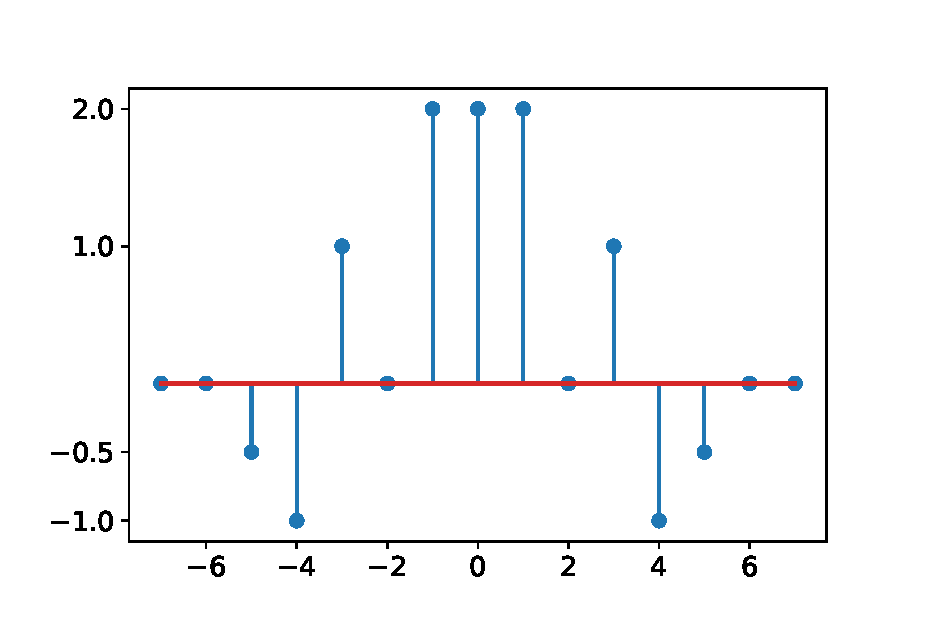
\includegraphics[width=100mm]{PSol10_Q3.eps}
\caption{
شکل مربوط به سوال 3 قسمت چ)
}
\end{figure}

\Q

الف)
$$
x[-n]\iff X(e^{-j\omega})
$$
در نتبجه
$$
y[n]=x[-n]\Big|_{n\to n-1}+x[-n]\Big|_{n\to n+1}\iff Y(e^{j\omega})=2X(e^{-j\omega})\cos \omega
$$
ب) 
$$
Y(e^{j\omega})=\Re\{X(e^{j\omega})\}
$$
پ)
\qn{
&X(e^{j\omega})=\sum x[n]e^{-j\omega n}\implies \\&X(e^{j\omega})e^{j\omega}=\sum x[n]e^{-j\omega (n-1)}\implies
\\&{d^2\over d\omega^2}X(e^{j\omega})e^{j\omega}=\sum -(n-1)^2x[n]e^{-j\omega (n-1)}\implies
\\&
[X''(e^{j\omega})-X(e^{j\omega})+2jX'(e^{j\omega})]e^{j\omega}
\\&=\sum -(n-1)^2x[n]e^{-j\omega (n-1)}\implies
\\&
(n-1)^2x[n]\iff X(e^{j\omega})-X''(e^{j\omega})-2jX'(e^{j\omega})
}{}
\Q

از شرط اول نتیجه می شود:
$$
{H(e^{j\omega})}{1\over 1-{1\over 4}e^{-j\omega}}=a+be^{-j\omega}
$$
یا به طور معادل
$$
{H(e^{j\omega})}=(a+be^{-j\omega})(1-{1\over 4}e^{-j\omega})
$$

همچنین چون طبق شرط سوم پاسخ فرکانسی با دوره‌ی $\pi$ متناوب است، باید ضریب 
$
e^{-j\omega}
$
 صفر باشد؛ پس
$$
b={1\over 4}a\implies {H(e^{j\omega})}=a(1+{1\over 4}e^{-j\omega})(1-{1\over 4}e^{-j\omega})=a(1-{1\over 16}e^{-2j\omega})
$$
و در نهایت از شرط دوم خواهیم داشت:
$$
a(1-{1\over 16}e^{-2j{\pi\over 2}})=1\implies a={16\over 17}
$$
در نهایت
$$
h[n]={1\over 17}(16-\delta[n-2])
$$
\Q

الف) 
\qn{
H(e^{j\omega})&={2-e^{-j\omega}\over (1+{1\over 2}e^{-j\omega})(1-{1\over 2}e^{-j\omega}+{1\over 4}e^{-2j\omega})}
\\&={2-e^{-j\omega}\over 1+{1\over 8}e^{-3j\omega}}
}{}
در نتیجه رابطه ورودی خروجی به صورت زیر است:
$$
y[n]+{1\over 8}y[n-3]=2x[n]-x[n-1]
$$
ب) با تعریف 
$
u=e^{-j\omega}
$:
\qn{
H(e^{j\omega})&={2-u\over 1+{1\over 8}u^3}=-8{u-2\over u^3+8}
\\&={A\over u+2}+{B\over u+2e^{j{\pi\over 3}}}+{C\over u+2e^{-j{\pi\over 3}}}
\\&={{8\over 3}\over u+2}+{-{4\over 3}\over u+2e^{j{\pi\over 3}}}+{-{4\over 3}\over u+2e^{-j{\pi\over 3}}}
\\&=
{{4\over 3}\over 1+{1\over 2}u}+
{-{2\over 3}e^{-j{\pi\over 3}}\over 1+{1\over 2}e^{-j{\pi\over 3}}u}+
{-{2\over 3}e^{j{\pi\over 3}}\over 1+{1\over 2}e^{j{\pi\over 3}}u}
}{}
در نتیجه
$$
h[n]={4\over 3}u[n]\Big\{
(-{1\over 2})^n-(-{1\over 2}e^{j{\pi\over 3}})^{n+1}-(-{1\over 2}e^{-j{\pi\over 3}})^{n+1}
\Big\}
$$
\Q

$$
H(e^{j\omega})={b+e^{-j\omega}\over 1-ae^{-j\omega}}
$$
در نتیجه
$$
|H(e^{j\omega})|^2={1+b^2+2b\cos\omega\over 1+a^2-2a\cos\omega}
$$
بنابراین 
$
b=-a
$
.

ب و پ)
\begin{figure}[h!]
\centering
\begin{subfigure}{0.49\textwidth}
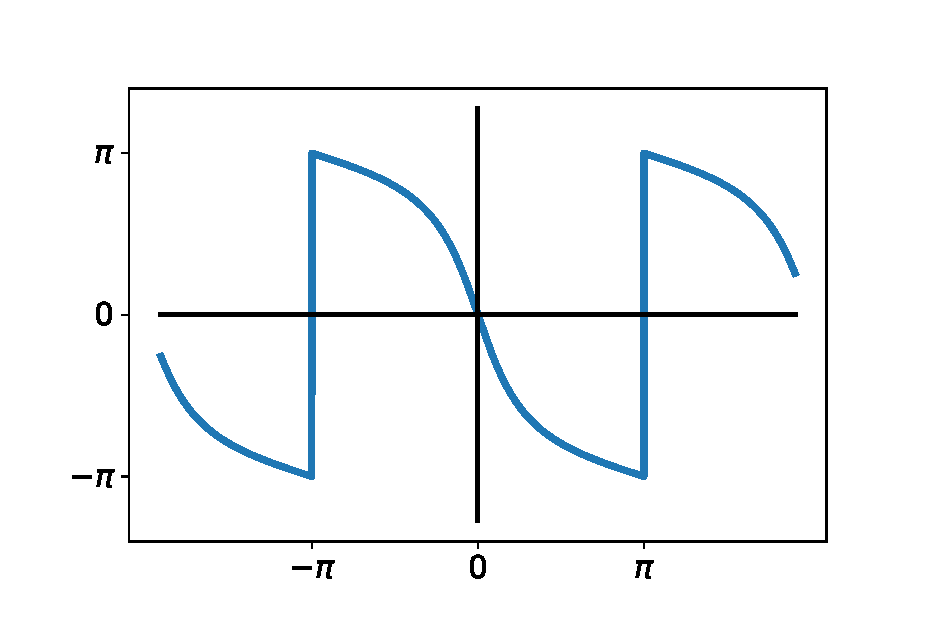
\includegraphics[width=80mm]{PSol10_Q7_1.eps}
\caption{$a={1\over 2}$}
\end{subfigure}
\begin{subfigure}{0.49\textwidth}
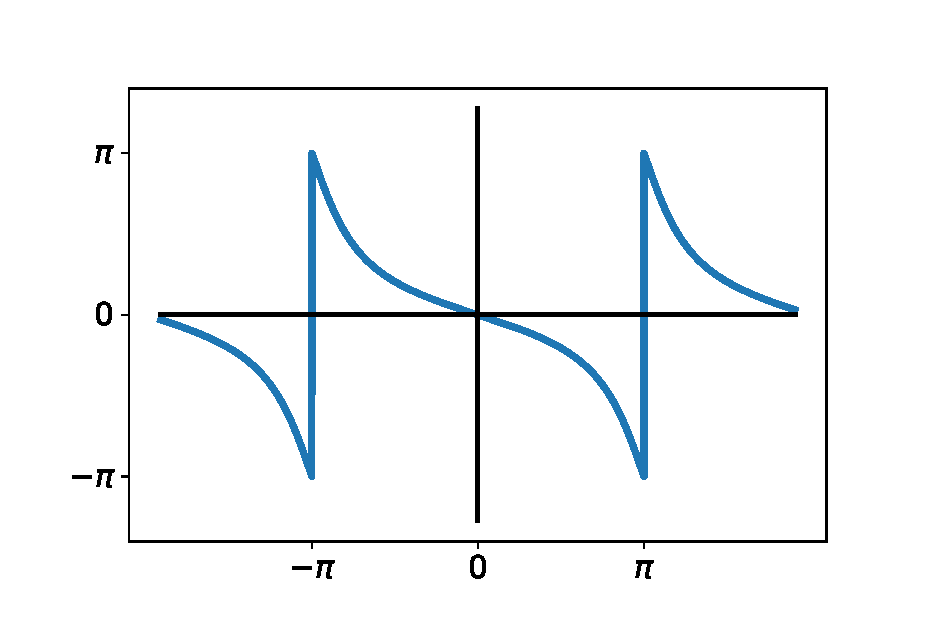
\includegraphics[width=80mm]{PSol10_Q7_2.eps}
\caption{$a=-{1\over 2}$}
\end{subfigure}
%\caption{
%شکل مربوط به سوال 3 قسمت چ)
%}
\end{figure}

ت)
\qn{
Y(e^{j\omega})&={{1\over 2}+e^{-j\omega}\over 1+{1\over 2}e^{-j\omega}}\cdot
{1\over 1-{1\over 2}e^{-j\omega}}
\\&={-{3\over 4}\over 1+{1\over 2}e^{-j\omega}}+
{{5\over 4}\over 1-{1\over 2}e^{-j\omega}}
}{}
بنابراین
$$
x[n]=u[n]\left\{{5\over 4}({1\over 2})^n-{3\over 4}(-{1\over 2})^n\right\}
$$
\begin{figure}[h!]
\centering
\begin{subfigure}{0.49\textwidth}
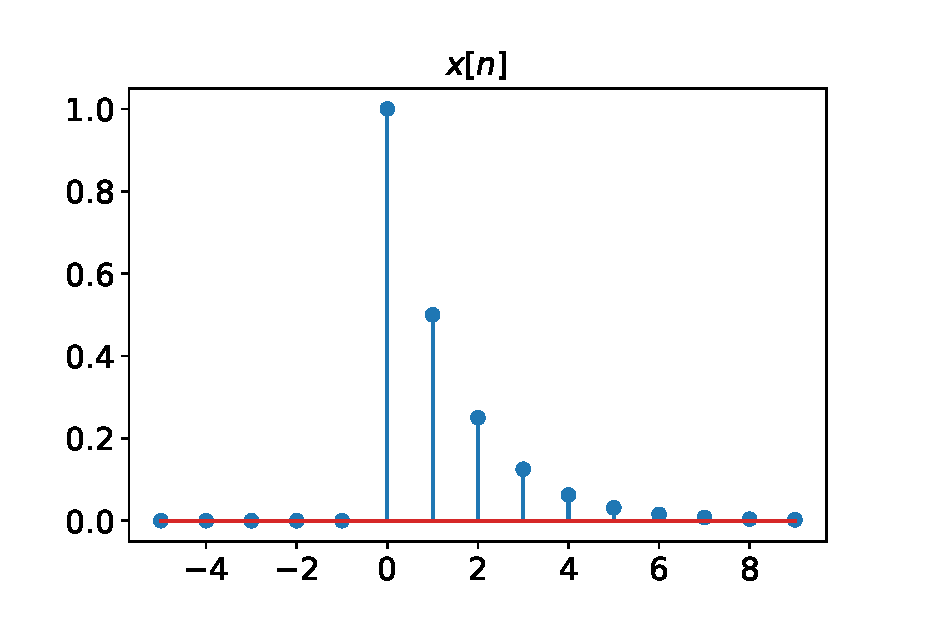
\includegraphics[width=80mm]{PSol10_Q7_4_1.eps}
%\caption{$a={1\over 2}$}
\end{subfigure}
\begin{subfigure}{0.49\textwidth}
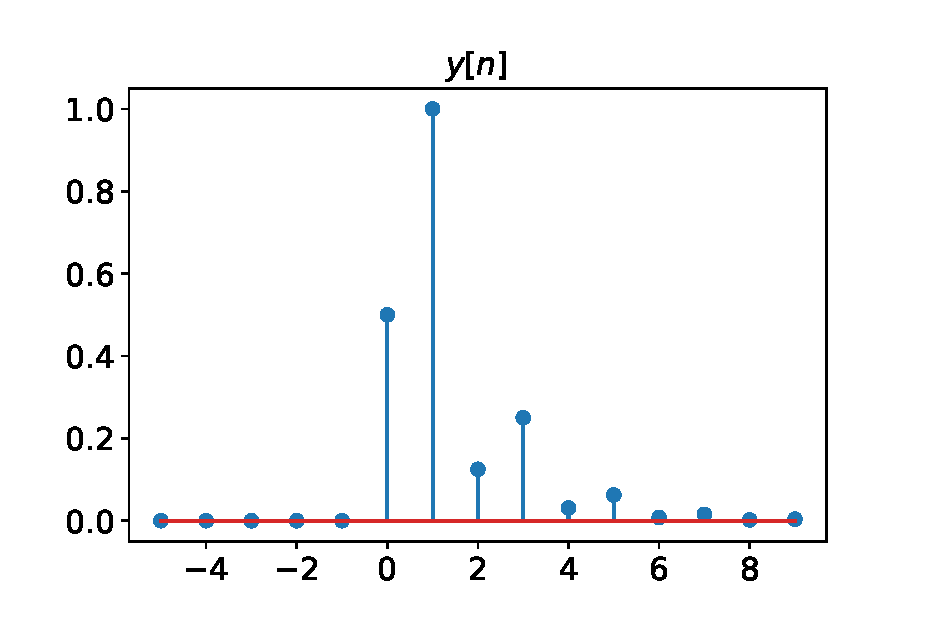
\includegraphics[width=80mm]{PSol10_Q7_4_2.eps}
%\caption{$a=-{1\over 2}$}
\end{subfigure}
%\caption{
%شکل مربوط به سوال 3 قسمت چ)
%}
\end{figure}

\Q

الف) به ازای 
$
\omega\ge 0
$
، پاسخ فرکانسی دارای اندازه‌ی 
$
\omega
$
 و فاز 
$
0
$
 و به ازای 
$
\omega< 0
$
، پاسخ فرکانسی دارای اندازه‌ی 
$
-\omega
$
 و فاز 
$
\pi
$
است؛ بنابراین
$$
H(e^{j\omega})=\omega , -\pi<\omega\le \pi
$$
ب)
$$
h[n]={1\over 2\pi}\int_{-\pi}^{\pi} \omega e^{j\omega n}d\omega=\begin{cases}
{2\pi\over jn}(-1)^n&,\quad n\ne0\\
0&,\quad n=0
\end{cases}
$$
\Q

الف)
$$
X(e^{j\omega})=X(e^{j(\omega-1)})\implies x[n]=x[n]e^{jn}
$$
از آنجا که جز در $n=0$ مقدار 
$
e^{jn}
$
 هیچگاه 1 نمی شود، در نتیجه داریم:
$$
x[n]=0\quad,\quad n\ne 0
$$
 و این گزاره درست است.

ب)
$$
X(e^{j\omega})=X(e^{j(\omega-\pi)})\implies x[n]=x[n]e^{j\pi n}=x[n](-1)^n
$$
از آنجا که در 
$
n=2k
$
 مقدار 
$
(-1)^n
$
 برابر 1 می شود، در نتیجه این گزاره نادرست است.

پ) از این تساوی نتیجه می شود که چون
$
X(e^{j\omega})
$
به دوره‌ی 
$
2\pi
$
 متناوب است، در نتیجه
$
X(e^{j{\omega\over 2}})
$
 نیز با دوره‌ی 
$
2\pi
$
متناوب بوده و داریم:
$$
X(e^{j{\omega+2\pi\over 2}})=X(e^{j({\omega\over 2}+\pi)})=X(e^{j{\omega\over 2}})=X(e^{j\omega})
$$
بنابراین
$$
{1\over2}X(e^{j({\omega\over 2})})+{1\over2}X(e^{j({\omega\over 2}+\pi)})=X(e^{j\omega})
$$
از طرفی می دانیم
\qn{
&x[2n]\iff {1\over2}X(e^{j({\omega\over 2})})+{1\over2}X(e^{j({\omega\over 2}+\pi)})
\\&x[2n+1]\iff {1\over2}e^{-j\omega}(X(e^{j({\omega\over 2})})-X(e^{j({\omega\over 2}+\pi)}))
}{}
بنابراین
\qn{
&x[n]=x[2n]
\\&x[2n+1]=0
}{}
که نتیجه می دهد 
$$
x[n]=0\quad,\quad n\ne 0
$$
و این گزاره درست است.

ت) می دانیم
\qn{
\begin{cases}
x[n/2]&,\quad n \text{زوج} \\
0&,\quad n \text{فرد} 
\end{cases}
\iff X(e^{2j\omega})
}{}
بنابراین
$$
x[n]=\begin{cases}
x[n/2]&,\quad n \text{زوج} \\
0&,\quad n \text{فرد} 
\end{cases}
$$
که مشابه همان قسمت قبل است؛ یعنی نمونه های فرد سیگنال صفر هستند و برای نمونه های زوج
$$
x[n]=x[2n]
$$
و به همین دلیل این گزاره نیز درست است.

\Q

الف-1) این سیستم خطی است زیرا عملیات های 
$
e^{-j\omega}X(e^{j\omega})
$
 و
$
{d\over d\omega}X(e^{j\omega})
$
  به ترتیب معادل با 
$
x[n-1]
$
و
$
-jnx[n]
$
 هستند که هر دو خطی اند؛ ولی چون عملیات 
$
-jnx[n]
$
تغییر پذیر با زمان است، در نتیجه کل سیستم خطی و تغییرپذیر با زمان می شود.

الف-2) به وضوح
$
X(e^{j\omega})=1
$
 بنابراین
$$
Y(e^{j\omega})=2+e^{-j\omega}
$$
و
$$
y[n]=2+\delta[n-1]
$$
ب) می توان نوشت:
$$
Y(e^{j\omega})=\int_{\omega-{\pi\over 4}}^{\omega+{\pi\over 4}}X(e^{j\omega})d\omega=\int_{-\pi}^{\pi}X(e^{j\theta})H(e^{j(\omega-\theta)})d\theta=
$$
که در آن:
$$
H(e^{j\omega})=\begin{cases}
1&,\quad |\omega|<{\pi\over 4}\\
0&,\quad {\pi\over 4}\le|\omega|\le \pi
\end{cases}
$$
بنابراین طبق خواص:
$$
y[n]=2 x[n]{\sin{\pi\over 4}n\over n}
$$
\Q

الف)
\qn{
&X(e^{j\omega})=\sum_n x[n]e^{-j\omega n}\implies 
\\& {d\over d\omega}X(e^{j\omega})=\sum_n -jnx[n]e^{-j\omega n}\implies 
\\&-jnx[n]\iff{d\over d\omega}X(e^{j\omega})
\\&nx[n]\iff j{d\over d\omega}X(e^{j\omega})
}{}
ب) سیگنال 
$
y[n]=\sum_{k=-\infty}^{n}x[k]
$
 خروجی سیستمی با پاسخ ضربه‌ی $u[n]$ و ورودی $x[n]$ است؛ از طرفی:
$$
u[n]\iff{1\over 1-e^{-j\omega}}+\pi\sum_{k=-\infty}^{\infty}\delta(\omega-2k\pi)
$$
بنابراین
\qn{
Y(e^{j\omega})&={X(e^{j\omega})\over 1-e^{-j\omega}}+\pi X(e^{j\omega})\sum_{k=-\infty}^{\infty}\delta(\omega-2k\pi)
\\&={X(e^{j\omega})\over 1-e^{-j\omega}}+\pi X(e^{j0})\sum_{k=-\infty}^{\infty}\delta(\omega-2k\pi)
}{}
%\qn{
%Y(e^{j\omega})&=\sum_{n=-\infty}^{\infty}\sum_{k=-\infty}^{n}x[k] e^{j\omega n}
%\\&=\sum_{k=-\infty}^{\infty}x[k]\sum_{n=k}^{\infty}e^{j\omega n}
%}{}
%سیگنال 
%$
%x[n]
%$
% را می توان به صورت مجموع 
%$
%x[n]=z[n]+X(e^{j0})
%$
%نوشت که 
%$
%z[n]
%$
% سیگنالی با DC صفر (یعنی 
%$
%Z(e^{j0})=0
%$
%)
%و 
%$
%X(e^{j0})
%$
% مقدار DC سیگنال
%$
%x[n]
%$
%است. از طرفی با تعریف
%$
%y[n]=\sum_{k=-\infty}^{n}x[k]
%$
%می توان نوشت:
%$$
%y[n]-y[n-1]=x[n]
%$$

پ) 
\qn{
&x[n]\iff X(e^{j\omega})\implies
\\&X(e^{j\omega})=\sum_n x[n]e^{-j\omega n}\implies
\\& X^*(e^{j\omega})=\sum_n x^*[n]e^{j\omega n}\implies
\\& X^*(e^{-j\omega})=\sum_n x^*[n]e^{-j\omega n}\implies
\\& x^*[n]\iff X^*(e^{-j\omega})
}{}
از آنجا که به دلیل حقیق بودن سیگنال داریم
$
x[n]=x^*[n]
$
 در نتیجه 
$
X(e^{j\omega})=X^*(e^{-j\omega})
$
.

اگر سیگنال حقیقی باشد؛ در این صورت:
\qn{
&x_e[n]={x[n]+x[-n]\over 2}={x[n]+x^*[-n]\over 2}\iff {X(e^{j\omega})+X^*(e^{j\omega})\over 2}=\Re\left\{X(e^{j\omega})\right\}
\\&x_o[n]={x[n]-x[-n]\over 2}={x[n]-x^*[-n]\over 2}\iff {X(e^{j\omega})-X^*(e^{j\omega})\over 2}=j\Im\left\{X(e^{j\omega})\right\}
}{}


ت) 
\qn{
\sum_n |x[n]|^2 &= {1\over 4\pi^2}\sum_n \int_{2\pi}\int_{2\pi} X(e^{j\theta_1})X^*(e^{j\theta_2}) e^{jn\theta_1}e^{-jn\theta_2}d \theta_1 d\theta_2
\\&= {1\over 4\pi^2}\sum_n \int_{2\pi}\int_{2\pi} X(e^{j\theta_1})X^*(e^{j\theta_2}) e^{jn\theta_1}e^{-jn\theta_2}d \theta_1 d\theta_2
\\&= {1\over 4\pi^2}\int_{2\pi}\int_{2\pi} X(e^{j\theta_1})X^*(e^{j\theta_2}) \sum_n e^{jn(\theta_1-\theta_2)}d \theta_1 d\theta_2
\\&= {1\over 4\pi^2}\int_{2\pi}\int_{2\pi} X(e^{j\theta_1})X^*(e^{j\theta_2}) 2\pi\delta(\theta_1-\theta_2)d \theta_1 d\theta_2
\\&= {1\over 2\pi}\int_{2\pi}\int_{2\pi} X(e^{j\theta_1})X^*(e^{j\theta_1}) \delta(\theta_1-\theta_2)d \theta_1 d\theta_2
\\&= {1\over 2\pi}\int_{2\pi}\int_{2\pi} |X(e^{j\theta_1})|^2 \delta(\theta_1-\theta_2)d \theta_1 d\theta_2
\\&= {1\over 2\pi}\int_{2\pi} |X(e^{j\theta_1})|^2 d \theta_1
}{}

ث) اگر ضرایب سری فوریه‌ی 
$
y(t)
$
 را با 
$
a_k
$ نشان دهیم، در این صورت:
\qn{
a_k&={1\over 2\pi} \int_{2\pi}y(t)e^{-j\omega_0 kt}dt
\\&={1\over 2\pi} \int_{2\pi}X(e^{jt})e^{-jkt}dt
\\&={1\over 2\pi} \int_{2\pi}X(e^{j\omega})e^{-jk\omega}d\omega
\\&=x[-k]
}{}
\end{document}